\begin{frame}{Fonctionnement de la librairie \texttt{keybert}}
\begin{enumerate}
\item entrée : un document
\item tokénisation du document en mots/phrases-clés candidates
\item génération des plongements du document et des mots/phrases-clés
\item calcul de la similarité cosinus document : mots/phrases-clés
\end{enumerate}
\begin{figure}
    \centering
    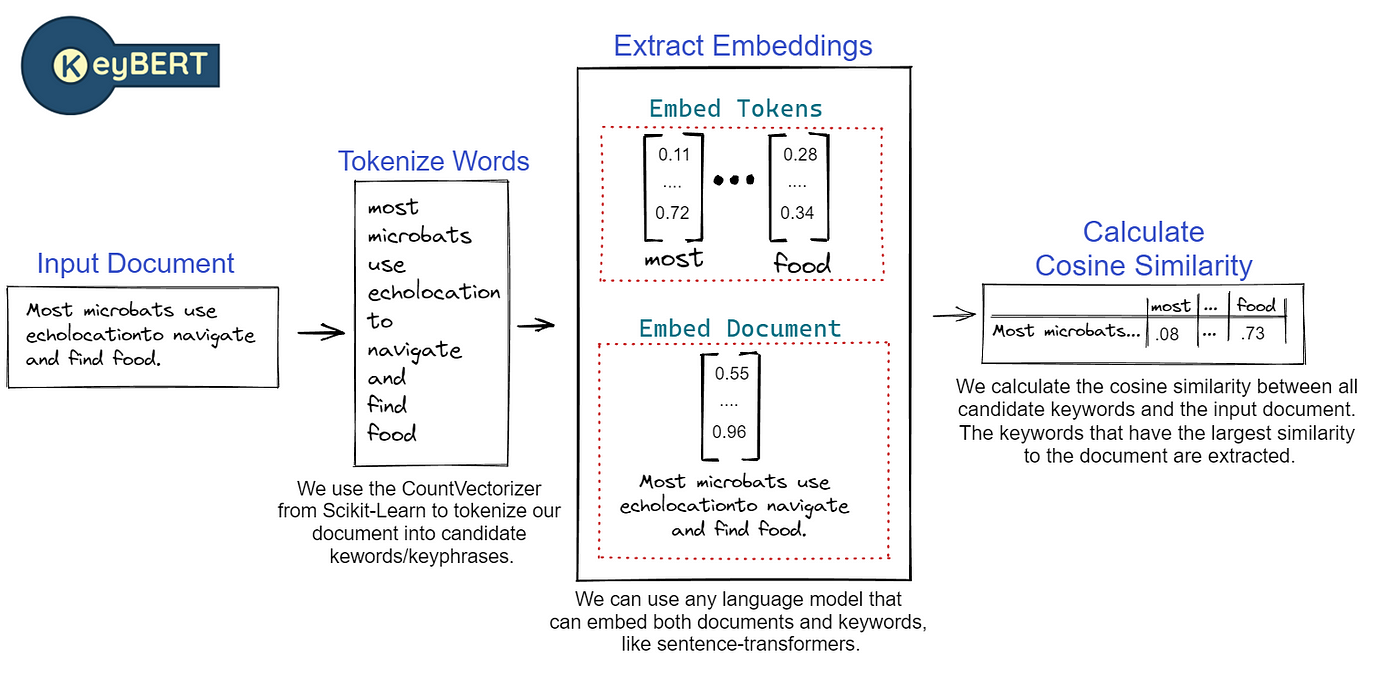
\includegraphics[width=80mm,scale=0.5]{pic/keybert.png}
    \caption{\textit{Pipeline} de la méthode \texttt{keybert} \citep{grootendorst2020keybert}.}
    \label{fig:enter-label}
\end{figure}
\end{frame}


\begin{frame}{\texttt{keybert} amélioré -- \textit{PatternRank}}
Key\textsc{BERT} + Keyphrase-Vectorizers = \textit{\textbf{PatternRank}} \hfill \citep{schopf2022}
\begin{itemize}
\item extraction des phrases-clés les plus similaires à un document
\item préservation de leur grammaticalité grâce aux motifs POS
\end{itemize}
\begin{figure}
    \centering
    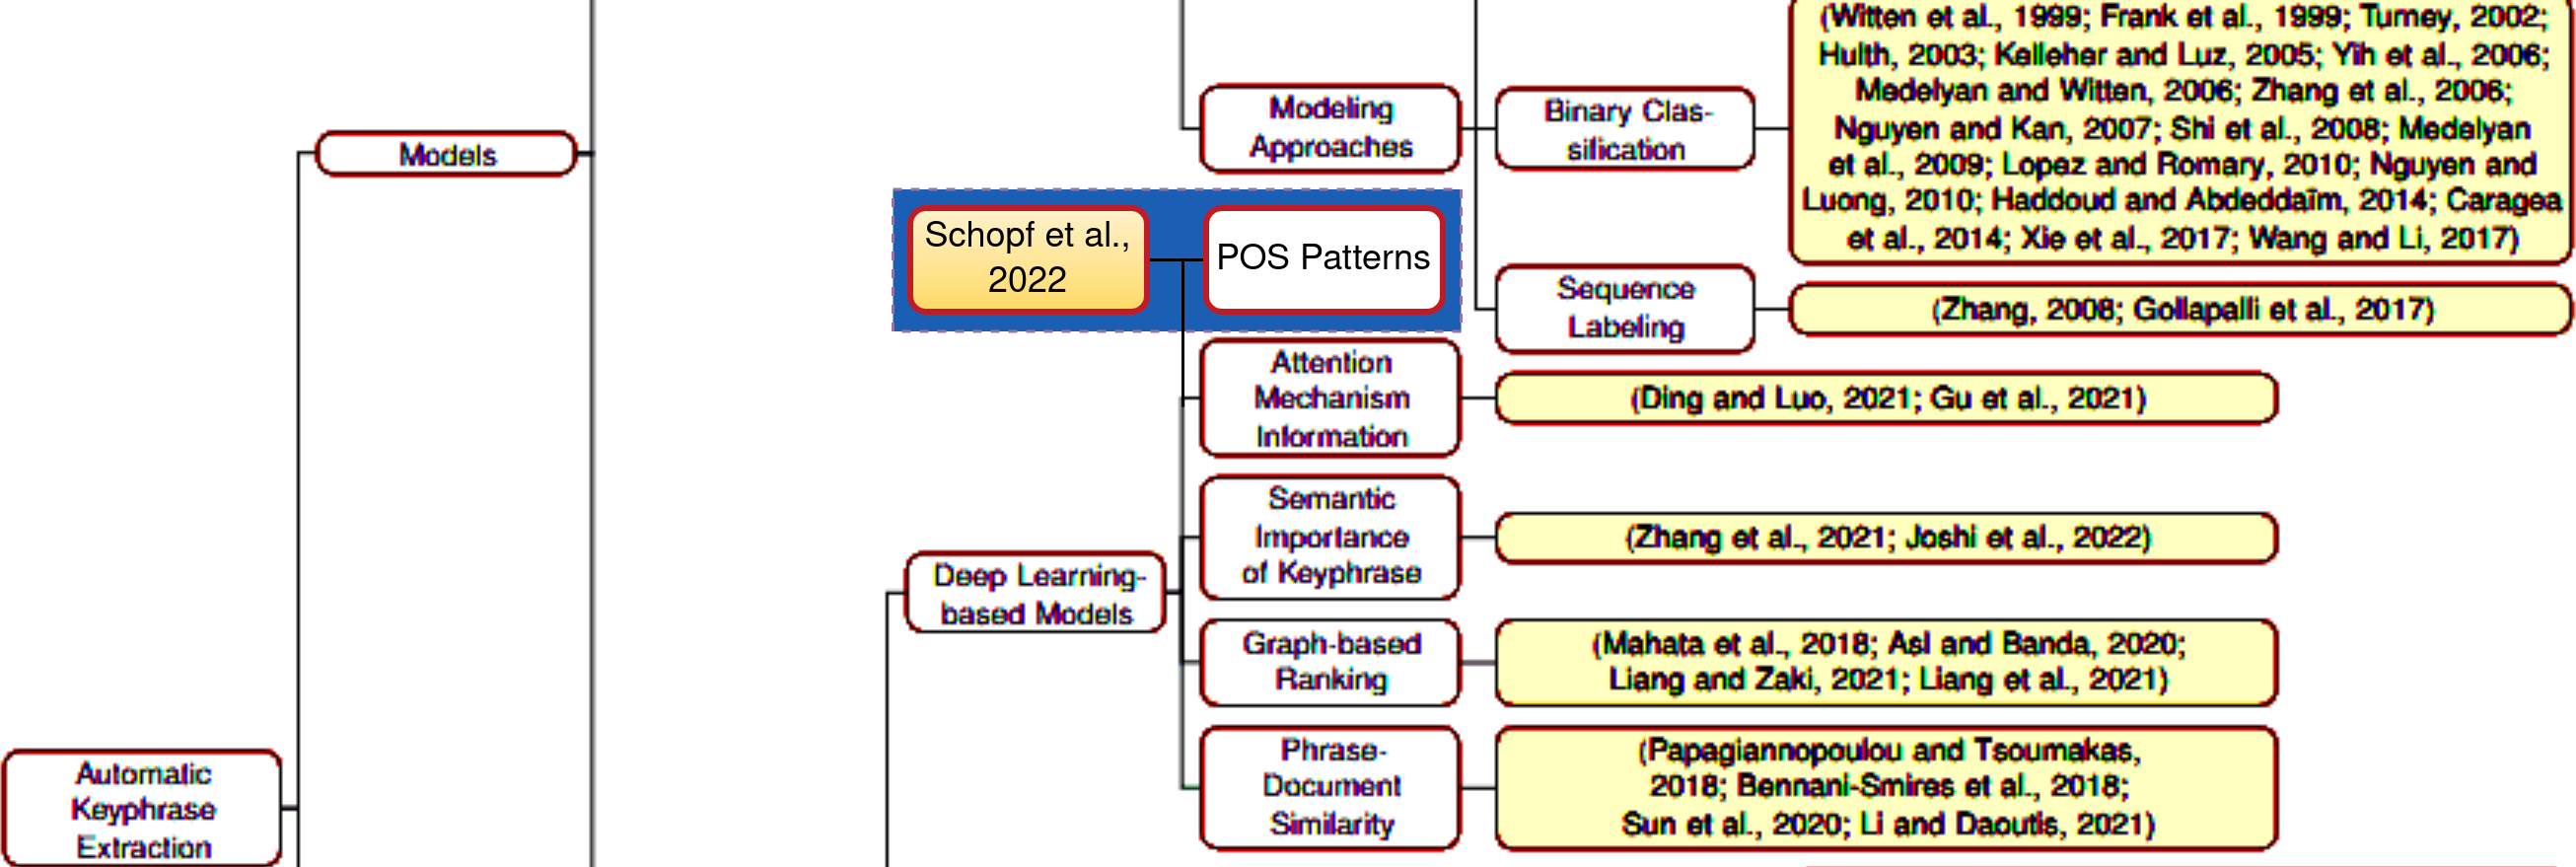
\includegraphics[width=110mm,scale=0.5]{pic/sota_lm_adapte.png}
    \caption{Extrait de l'état de l'art sur l'extraction des mots-clés, adapté de \citet{xie2023}}
    \label{fig:enter-label}
\end{figure}
\notecite{schopf2022}
\end{frame}

\begin{frame}{Fonctionnement de la méthode \textit{PatternRank}}
%\begin{itemize}
%\item extraction des phrases-clés non-supervisée
%\item exploite des modèles de langues pré-entraînés + parties du discours
%\end{itemize}
\begin{enumerate}
\item entrée : un seul document texte tokenisé
\item étiquetage des tokens avec les balises POS
\item sélection des tokens correspondant au modèle POS défini comme phrases-clés candidates
\item génération des plongements du document et des phrases-clés candidates par un modèle de langue
\item calcul des similarités cosinus entre les plongements du document et des phrases-clés candidates + classement des phrases-clés
\item extraction des \textit{N} phrases-clés les plus représentatives
\end{enumerate}
\begin{figure}
    \centering
    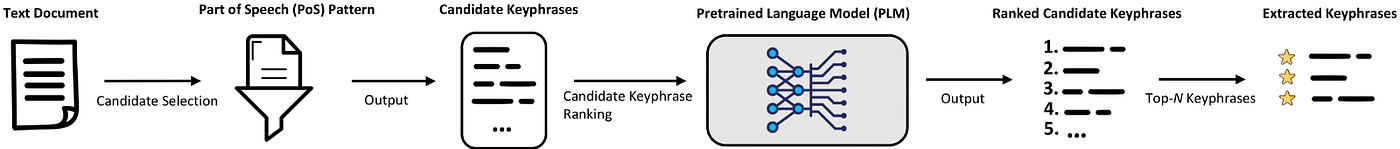
\includegraphics[width=110mm,scale=0.5]{pic/patternrank_workflow.png}
    \caption{\textit{Workflow} de la méthode \textit{PatternRank}.}
    \label{fig:enter-label}
\end{figure}
\end{frame}